%Punchline!

%make plot of delta [C/N] versus R0(1D), color code observed binned points by mass of the star

Given the measured amounts of mixing described in Section \ref{sec:obs} and the reduced density ratios computed for stars of various masses and metallicities described in Section \ref{sec:mesa_results}, it is now possible to compare the observed amounts of extra mixing to the predictions of various thermohaline models from Section \ref{sec:formalism}, and determine if the observed mixing is at least qualitatively consistent with the expectations of the thermohaline instability. We show in Figure \ref{Fig:punchline} the corrected changes in [C/N] compared to the inferred reduced density ratios, in an orientation analogous to the theoretical predictions shown in Figure \ref{fig:parameterization_compare}. We note that the observed trends are not strongly sensitive to the assumed mixing model, with increasing mixing at lower reduced density ratios no matter which parameterization is chosen. 




Interestingly, the data seem to have some similarities and some differences compared to the theoretical lines, shown again in Figure \ref{Fig:compare} for comparison. The observed amounts of mixing are strongly correlated with the fluid parameters as predicted, even for stars with different masses and metallicities but similar reduced density ratios, consistent with theoretical predictions, under the simplifying assumption that the mixing efficiency and magnetic field are not varying strongly with mass or metallicity. We note a decrease in the amount of mixing as the density ratio increases, which is consistent with standard prescriptions of mixing but inconsistent with magnetohydrodynamic models that include strong magnetic fields. We also note that the range of reduced density ratios probed here by the observed data is much smaller than the range of density ratios simulated in the theoretical community, suggesting that focusing simulations on the relevant range might be beneficial. %, assuming the density ratios inferred in this paper are assumed correctly.   

%note that the scatter is also important here- if the mixing actually depends on B field, and that depends randomly on the star (or on the stellar M/Z combo on average), then stars of the same R0 should have a range of mixi-ness. If R0 is the only parameter that matters, then mixing should strongly correlate with R0 with only minimal/ observational measurement scatter. 

%FIGURE solar---------------------------------------------------
\begin{figure*}[!tb]
\begin{center}
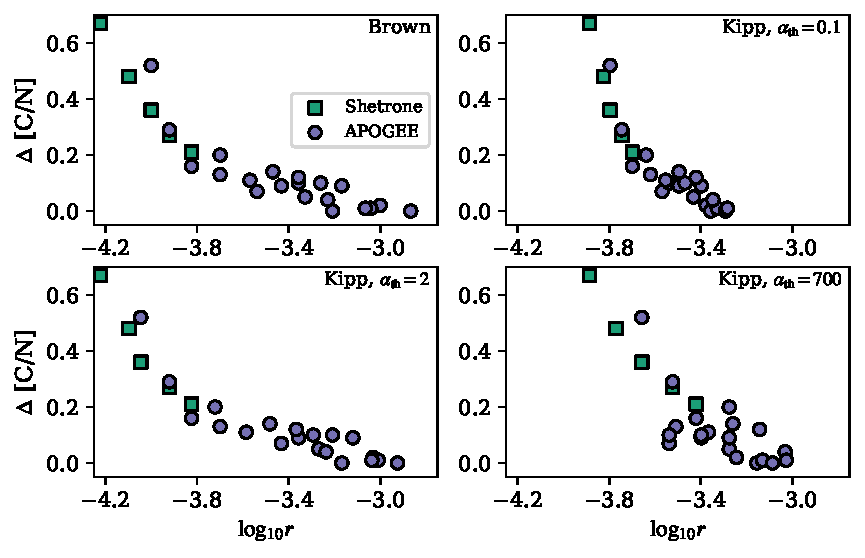
\includegraphics[width=\textwidth]{./figures/mixing_vs_r/mixing_vs_r.pdf}%[width=9cm, clip=true, trim=1in 1in 1in 1in]{./Figs/omgcomp.eps}
\caption{Corrected measurements of the change in [C/N] near the red giant branch bump, compared to the reduced density ratio inferred from one-dimensional models using various thermohaline mixing prescriptions (Brown, Kippenhahn $\alpha=0.1$, Kippenhahn $\alpha=0.2$,Kippenhahn $\alpha=0.700$), color coded by the metallicity bin of each data point. In general there is a clear correlation between these parameters, suggesting that the observed mixing is related to fluid instabilities. More mixing is observed when the fluid is more unstable to the thermohaline instability, consistent with standard theories of thermohaline mixing, and observations do not probe high values of the reduced density ratios where magnetic fields may be important.
\label{Fig:punchline}
}
\end{center}
\end{figure*}

\begin{figure*}[!tb]
\begin{center}
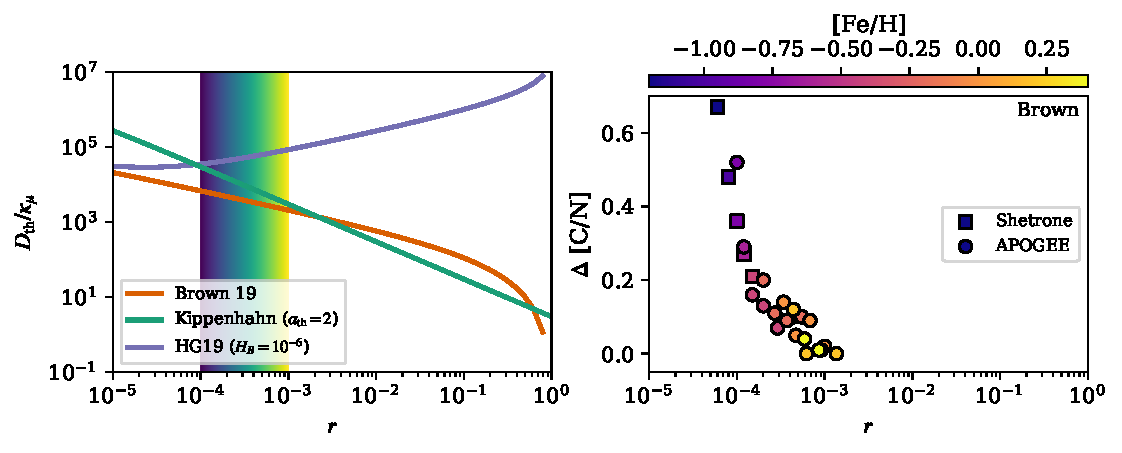
\includegraphics[width=\textwidth]{./figures/punchline/punchline.pdf}
\caption{Left: A reproduction of Figure \ref{Fig:bothmodels} showing the predicted amount of mixing on the y-a}
\label{Fig:compare}
\end{center}
\end{figure*}


